\documentclass{article}\usepackage[]{graphicx}\usepackage[]{color}
%% maxwidth is the original width if it is less than linewidth
%% otherwise use linewidth (to make sure the graphics do not exceed the margin)
\makeatletter
\def\maxwidth{ %
  \ifdim\Gin@nat@width>\linewidth
    \linewidth
  \else
    \Gin@nat@width
  \fi
}
\makeatother

\definecolor{fgcolor}{rgb}{0.345, 0.345, 0.345}
\newcommand{\hlnum}[1]{\textcolor[rgb]{0.686,0.059,0.569}{#1}}%
\newcommand{\hlstr}[1]{\textcolor[rgb]{0.192,0.494,0.8}{#1}}%
\newcommand{\hlcom}[1]{\textcolor[rgb]{0.678,0.584,0.686}{\textit{#1}}}%
\newcommand{\hlopt}[1]{\textcolor[rgb]{0,0,0}{#1}}%
\newcommand{\hlstd}[1]{\textcolor[rgb]{0.345,0.345,0.345}{#1}}%
\newcommand{\hlkwa}[1]{\textcolor[rgb]{0.161,0.373,0.58}{\textbf{#1}}}%
\newcommand{\hlkwb}[1]{\textcolor[rgb]{0.69,0.353,0.396}{#1}}%
\newcommand{\hlkwc}[1]{\textcolor[rgb]{0.333,0.667,0.333}{#1}}%
\newcommand{\hlkwd}[1]{\textcolor[rgb]{0.737,0.353,0.396}{\textbf{#1}}}%

\usepackage{framed}
\makeatletter
\newenvironment{kframe}{%
 \def\at@end@of@kframe{}%
 \ifinner\ifhmode%
  \def\at@end@of@kframe{\end{minipage}}%
  \begin{minipage}{\columnwidth}%
 \fi\fi%
 \def\FrameCommand##1{\hskip\@totalleftmargin \hskip-\fboxsep
 \colorbox{shadecolor}{##1}\hskip-\fboxsep
     % There is no \\@totalrightmargin, so:
     \hskip-\linewidth \hskip-\@totalleftmargin \hskip\columnwidth}%
 \MakeFramed {\advance\hsize-\width
   \@totalleftmargin\z@ \linewidth\hsize
   \@setminipage}}%
 {\par\unskip\endMakeFramed%
 \at@end@of@kframe}
\makeatother

\definecolor{shadecolor}{rgb}{.97, .97, .97}
\definecolor{messagecolor}{rgb}{0, 0, 0}
\definecolor{warningcolor}{rgb}{1, 0, 1}
\definecolor{errorcolor}{rgb}{1, 0, 0}
\newenvironment{knitrout}{}{} % an empty environment to be redefined in TeX

\usepackage{alltt}
\IfFileExists{upquote.sty}{\usepackage{upquote}}{}
\begin{document}

\title{Climate Prediction Markets and Convergence of Predictive Models}
\author{not sure about the author order}

\maketitle
	
%%%%%%%%%%%%%%%%%%%%%%%%%%%%%%%%%%%%%%%%%%%%%%%%%%%%%%%%%%%%%%%%%%%%%%%%%%%%%%%%
\section*{Abstract}
We present an agent-based model of a climate prediction market in which traders adapt their belief about the climate based on the monetary performance of their neighboring traders in a social network. We analyze the model to determine how a variety of factors affect whether climate prediction markets foster a convergence of market participants' beliefs regarding a true model of the earth's climate. We find that only the imposed ``true model'' itself significantly affects the convergence of beliefs. If the true model from which the temperature data is generated is auto-regressive, with no human-induced effects, participation in the prediction market, on average, does not cause convergence of traders' beliefs. On other hand, if anthropogenic climate change is real, traders' beliefs are more likely than not to converge toward the correct climate model due to participation in the market.

%%%%%%%%%%%%%%%%%%%%%%%%%%%%%%%%%%%%%%%%%%%%%%%%%%%%%%%%%%%%%%%%%%%%%%%%%%%%%%%%
\section*{Introduction}
	
The previous two decades saw a strong polarization of the climate change debate. Although the scientific consensus on the anthropogenic nature of climate change strongly increased, the average belief about anthropogenic climate change did not evolve much within the public \cite{Vandenbergh2013f}. In addition, the divide on anthropogenic climate change between liberals and conservatives has grown steadily, indicating that the question is becoming increasingly politicized and potentially disconnected from scientific evidence. This is troubling given the costs of a misinformed climate policy. If anthropocentric climate change is a myth but is taken to be true, a tremendous amount of public resources will be wasted on adaptation and mitigation efforts. On the other hand, if climate change is human induced but not recognized as so, the costs of inaction would be huge. Given that effective climate policies require long-lasting measures to be taken, the importance of an accurate consensus on the issue is manifest.
	
Attempts to foster such consensus face many social and psychological challenges. Recently, people have argued that such challenges could be met by setting up climate prediction markets \cite{Hsu2011,Vandenbergh2013f}. The idea of using prediction markets to efficiently aggregate information about uncertain events has been discussed for decades \cite{Horn2014c}. Prediction markets have been shown to have interesting theoretical properties \cite{Set1998,Hanson2012} and to perform well in terms of prediction accuracy in experiments \cite{Hanson2006,Healy2010}, agent-based models (ABM) \cite{Klingert2012c,Jumadinova2011a}, and in the real-world \cite{Wolfers2006}.

% NOTE: the follwing two paragraphs is some good lit reivew, but whether it is included in the main article text depends on the potential journal we are submitting to. journals like science and nature do not want lit review, or claims to priority. So, do not delete these following two paragraphs that are commented out until we are accepted into a journal that doesnt want this. For Nature CC we could put this in an SI Appendix.

% \cite{Tseng2010a} study an ABM of a continuous double auction model with various types of market strategies (including two variants of the zero-intelligence agents). They compare the behavior of their simulation with data from a prediction market for the outcome of political elections. They find that despite their simplicity, zero-intelligence agents capture some salient features of real market data. \cite{Klingert2012c} reach similar conclusions with respect to experimental data from  \cite{Hanson2006}. In their simulation, \cite{Klingert2012c} compare continuous double auctions with logarithmic market scoring rules and find that the latter generally outperform continuous double auctions in terms of prediction accuracy. In some variants of the two last models, agents' strategies feature learning, but these are rather basic and unrelated to a formal predictive model. 
% 	
% \cite{Jumadinova2011a} conducted research more similar to our project, as they explicitly include information about uncertain events in their model. The paper studies a continuous double auction model in which agents update their beliefs about the uncertain events based on information on the event. New beliefs are modeled as a weighted sum of the last period's beliefs and market prices. The agent's information set changes every period. The better the information set, the more likely the agent is to put higher weights on last period's prices when revising their beliefs. Not much structure is imposed on the information set and the way it is used to generate the weights in the update function. Therefore, the model does not allow for investigating the convergence of predictive models. \cite{Ontanon2009} study the effect of deliberation on a simulated prediction market. They assume that agents use Case-Based Reasoning \cite{Aamodt1994} to debate about  uncertain outcomes with their neighbors in a social network.  Although the model could in theory be used to assess convergence of predictive models by looking at the arguments agents adopt after the deliberation, this is not done by the authors. Also, the way beliefs are formed and revised through argumentation is rather abstract and might not be ideal to study climate prediction markets.

However, to the best of our knowledge, the idea that prediction markets can generate consensus \emph{on the factors} affecting  uncertain events has never been quantitatively explored. ABMs of prediction markets have been studied \cite{Klingert2012c,Tseng2010a,Jumadinova2011a}, some of which feature communication between agents. In these models, however, beliefs about the uncertain outcomes are constructed in rather abstract ways. In particular, beliefs are not based on structural models from which agents could derive causal implications, and therefore these models are not suitable for investigating the convergence of the underlying explanatory models agents employ for prediction.

From a public policy perspective, changing the explanatory models of market participants is one of the most important roles that prediction markets might play.\footnote{and perhaps the most important potential social benefit of prediction markets given the comparable predictive power of statistical models, which are less expensive than setting up and maintaining prediction markets \cite{goel_prediction_2010}.} Effective climate policy not only requires an accurate consensus on future climate \emph{outcomes}. It also requires an accurate consensus on the causal \emph{mechanisms} influencing such outcomes. If people agree that temperature will rise, but some believe it will be due to greenhouse gases, while others believe that it will be caused by increased solar activity, inconsistent and ineffective policies may be implemented. Our model is designed to investigate whether, and under what conditions, prediction markets can foster such convergence in predictive models.

%%%%%%%%%%%%%%%%%%%%%%%%%%%%%%%%%%%%%%%%%%%%%%%%%%%%%%%%%%%%%%%%%%%%%%%%%%%%%%%%
\section*{Model Design}

TODO: Martin use this text below (it is commented out) from the original document and flesh it out for the Supplementary Material and then write a couple paragraph summary and the key equations to put in this main article right here.

In particular, lets go over main design and then define what each of these mean in our model: 	
\begin{itemize}
	\item \texttt{ideo} $\sim Unif(0,1)$
	\item \texttt{market.complet} $\sim Unif(0,1000)$ (mapped into integer)
	\item  \texttt{n.edge} $\sim Unif(100,200)$ (mapped into integer)
	\item  \texttt{n.traders} $\sim Unif(50,250)$ (mapped into integer)
	\item \texttt{risk.tak}  $\sim Unif(0,1)$
	\item  \texttt{seg} $\sim Unif(0,1)$
	\item  \texttt{true.model} $\sim Binom(0.5)$
\end{itemize}

% 	\section{Model}
% 	
% 	\label{model}
% 	
% 	In its current form, the ABM is composed of the following elements.
% 	
% 	\begin{description}
% 		\setlength\itemsep{0em}
% 		\item [A simple ``true" model $F$ of world temperatures.] The model is an additive autoregressive function and is taken  from \cite{Sumner2008b} (it is a simplified version of  RICE99 from \cite{Nordhaus}).
% 		\begin{align}
% 		\label{true}
% 		\begin{split}
% 				T_t ~ =~  \lambda T_{t-1} + \beta \underbrace{\big[ \kappa GHG_{t-1} - \alpha P_t^{1/2} + \delta Y_t  \big]}_{\equiv GHG_t} \\
% 				- \rho \underbrace{\big[ \omega G_{t-1} + \theta X_{t} \big]}_{\equiv G_t} +  \epsilon_t, 
% 		\end{split}
% 		\end{align}
% 		where
% 		\begin{itemize}
% 			\item $T_t$ is the temperature at time $t$,
% 			\item $GHG_t$ are greenhouse gas emissions at time $t$,
% 			\item $P_t$ are spendings in policies alleviating climate change at $t$,
% 			\item $Y_t$ is time $t$'s world Gross Domestic Product (GDP),
% 			\item $G_{t}$ is the effect in period $t$ of geo-ingeneering produced before $t$. 
% 			\item $X_t$ are spending in geo-ingeneering in period  $t$.
% 		\end{itemize}
% 		
% 		
% 		\item[ Beliefs.]  Traders use $5$ models to  forecast future temperatures in order to trade on the prediction market. These $5$ models are interpreted as the trader's beliefs about the true climate model.  Again, these models are taken from \cite{Sumner2008b}). They are meant to represent pervasive positions on climate change in the public debate. Four of these models are approximations of the true model in \eqref{true} described below, and one of them is the true model itself.\footnote{Thus some traders use the true model to make predictions. This does not mean that traders using the true model make perfectly accurate predictions. Although these traders believe in the correct \emph{functional form} of the model, they still need to calibrate it based on limited noisy data. Therefore, the values they use for  the \emph{parameters} of the model will typically still be off.} 
% 		
% 		\begin{enumerate}
% 			\setlength\itemsep{0em}
% 			\item Anthropogenic climate change is a myth ($\beta = \rho = 0$),
% 			\begin{align}
% 			T^1_t = \lambda T_{t-1} +  \epsilon_t.
% 			\end{align}
% 			\item Anthropogenic climate change is real but policies and geoengineering are ineffective ($\omega = \rho = 0$),
% 			\begin{align}
% 			T^2_t & = \lambda T_{t-1} + \beta \big[ \kappa GHG_{t-1}  + \delta Y_t  \big] +  \epsilon_t.
% 			\end{align}
% 			\item Anthropogenic climate change is real, policies are effective, but not geoengineering ($\rho = 0$),
% 			\begin{align}
% 			T^3_t = \lambda T_{t-1} + \beta \big[ \kappa GHG_{t-1} - \alpha P_t^{1/2} + \delta Y_t  \big] +  \epsilon_t.
% 			\end{align}
% 			\item Anthropogenic climate change is real, policies are ineffective, but geoengineering works($\alpha = 0$),
% 			\begin{align}
% 			\begin{split}
% 		T^4_t = \lambda T_{t-1} + \beta \big[ \kappa GHG_{t-1} + \delta Y_t  \big]\\ - \rho \big[ \omega G_{t-1} + \theta X_{t} \big] +  \epsilon_t.
% 			\end{split}
% 			\end{align}
% 			
% 		\end{enumerate}
% 		
% 		\item[ Traders.] Traders are endowed with some initial money in an Experimental Currency Unit (ECU), and an initial approximate model. Approximate models are distributed at random among the traders with each model having the same probability of being assigned to any trader.  Traders use the distribution of temperatures obtained from their approximate models to determine their reservation price for different securities. 
% 		
% 		Securities pay 1 ECU  if the actual temperature at some time $t^*$ falls between a certain range. Traders are assumed to be \emph{risk-neutral expected utility maximizers}. Therefore, their reservation price for a security $\tilde{s}$ is simply their assessment of the probability that the temperature at time $t^*$ falls in the range covered by $\tilde{s}$.
% 		
% 		  Based on their reservation price, traders behave as ``\emph{zero-intelligence}" agents \citep{Gode1993}, that is they sell at a random price above their reservation, and buy at a random price below their reservation. These strategies are simple but have been shown to provide good approximations of the behavior of prediction markets (see for instance \cite{Klingert2012c}), and financial markets more broadly. 
% 		  
% 		\item[Continuous-Double Auction (CDA) market structure.] Continuous-Double auctions ( or some variants thereof) are common \emph{market mechanisms}, i.e. procedures to match buy and sell orders. CDA are notably used on large stock markets (see for instance \cite{Tseng2010a}). Our model features a particular version of CDA (more in section \ref{implem}). 
% 		
% 		\item[A social network.] Traders are part of a social network. Every time a security is realized, each trader $i$ looks at the performance of their neighbors in the network. If one of $i$'s neighbors, say $j$, is richer than $i$, $i$ interprets this has an indication that $j$ has a better approximate model. Then $i$ considers adopting $j$'s approximate model.\footnote{Traders start with the same initial amount of money, so differences in money among traders can only come from  traders' interactions through the market.} 
% 		
% 		An example of such social network is depicted in Figure \ref{socnet}. This corresponds to the initial social network for some of our simulations. The color of the nodes identify the approximate model of the trader. Notice the belief-homophily of the initial network which can be seen by the high clustering of traders with the same approximate model. Although traders can change their approximate model (i.e. colors can change in the graph), the connections between traders do not change as the market unfolds (i.e. the edges are fixed).
% 	\end{description}
% 	
% 	\begin{figure}
% 		\begin{center}
% 		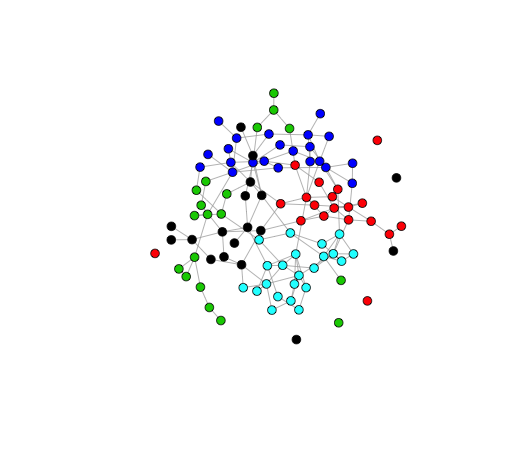
\includegraphics[scale = 0.5]{network.png}
% 		\end{center}
% 		\caption{An example of the initial state of a belief network \label{socnet}}
% 	\end{figure}
% 	
% 	\subsubsection*{Timing}
% 	
% 	The time periods $t$ are grouped in trading \emph{sequences}. In a given sequence, the potential payments associated with traded securities are all based on the temperature at the end of the sequence. For instance, the third trading sequence might start in period $t=300$ and end in period $t = 399$. In this case, a security traded in the third sequence pay 1 ECU if the temperature at $t=400$ falls into the range of temperatures covered by the security. 
% 	
% 	   At each time $t$, traders are assumed to know the past value of the temperature $T_{0:t}$ and the vector of past explanatory variables $Z_{0:t}$. In a sequence finishing at time $t^*$,  traders also have common knowledge of $Z_{t:t^*}$, the future values of explanatory variables up to $t^*$. However, at any $t$, traders do not know the value of any future temperatures. In particular, in a given sequence, traders do not know the value of $T_{t^*}$. Traders can only predict $T_{t^*}$ using their approximate model and their knowledge of $Z_{t:t^*}$. Notice that because $Z_{t:t^*}$ is common knowledge, in each period $t$ every trader $i$ with the same approximate model forms the same expectation 
% 	   \begin{align*}
% 	  \mu_{ti} \equiv E_t( T_{t^*} ~|~ T_{0:t}, Z_{t:t^*},  \text{ approximate model of } i \text { at } t).
% 	   \end{align*}
% 	   We assume that the probability density that trader $i$ associate with $T_{t^*} = \tilde{T}$ at any $t$ is
% 	   \begin{align*}
% 	   f_{it}(T) = \mu_{ti} + N(0, \sigma_T),
% 	   \end{align*}
% 	   
% 	   where $N$ stands for a normal distribution and $\sigma_T$ is a fixed number determined by the true variance of temperatures.       
% 	   
% 	    At each time $t$, traders
% 	\begin{itemize}
% 		\setlength\itemsep{0em}
% 		\item recalibrate their approximate model based on the new set of past data available at $t$,
% 		\item compute their belief-density for $T_{t^*}$ and use it to determine the expected value they attached to each security,
% 		\item and trade on the market based on their market strategy at $t$.
% 	\end{itemize}
% 	
% 	
% 	At $t^*$, when the sequence ends, there is only one security $s^*$ associated with a range of temperatures including the actual $T_{t^*}$. Thus,
% 	\begin{itemize}
% 			\setlength\itemsep{0em}
% 		\item traders receive 1 ECU per unit of $s^*$ they own, and
% 		\item  consider adapting their approximate model as described above.
% 	\end{itemize}
% 	
% 	\section{Implementation}
% 	\label{implem}
% 	The model is implemented in the \texttt{R} programming language,  using the \texttt{igraph} package to model the social network. Each trader in the model is a node of an \texttt{igraph} network. Because the model uses time-series data and  traders calibrate statistical models based on these data, \texttt{R}, primarily used for statistical computing, is particularly convenient. 
% 	
% 	 Traders calibrate their approximate models based on past-data using Pooled Ordinary Least Squares. This is questionable from a statistical point of view, but provides an approximation of the way traders may form their forecast on actual prediction markets. Because the model is in \texttt{R}, it is also very easy to change the estimation method or model to virtually any statistical model, and the effect of altering models may easily be studied in the future.
% 	
% 	 In each period $\tilde{t}$, our version of the CDA works as follows.
% 	
% 	\begin{enumerate}
% 			\setlength\itemsep{0em}
% 		\item Every trader $i$ choses at random a security $s_i^B$ she will try to buy.
% 		\item Every trader $i$ also chooses at random a security $s_i^S$ she will try to sell among the securities she owns a positive amount of (if any).
% 		\item Traders then decide of their selling $p_i^S$ and buying price $p_i^S$. They do so based on their believed-density of temperatures at the end of the sequence, and following the zero-intelligence rule described above.
% 		\item Traders go to the market one at the time, in a random order.
% 		\item When $i$ comes to the market, she place \emph{limit orders} in the order book. These orders  specify that $i$ is willing to buy $s_i^B$ at  any price below $p_i^B$, and to sell $s_i^S$ at any price above $p_i^S$.
% 		\item The market maker then tries to match $i$'s orders with some order which was put in the order book \emph{before} $i$ came to the market.
% 		\item If there are  outstanding sell offers for $s_i^B$ at price $p$ lower than $p_i^B$, then a trade is concluded. Trader $i$ buys one unit from the sellers who sells at the \emph{highest} price below $p_i^B$, and the sell and buy offers are removed from the order book.
% 		\item If there are  outstanding buy offers for $s_i^S$ at price $p$ higher than $p_i^S$, then a trade is concluded. Trader $i$ sells one unit to the buyer who buys at the \emph{highest} price above $p_i^S$, and the  sell and buy offers are removed from the order book.
% 		\item Whenever all traders have come to the market, any remaining outstanding offer is removed from the order book, and the trading period is concluded. 
% 	\end{enumerate} 
% 	
% The model depends on the following parameters. 
% \begin{description}
% 	\setlength\itemsep{0em}
% 	\item[Network parameters.]~
% 	\begin{description}
% 			\setlength\itemsep{0em}
% 		\item [\texttt{n.traders}:] the number of traders.
% 		\item [\texttt{n.edg} :] the number of edges in the social network. This number is fixed throughout the experiments.   
% 		\item [\texttt{seg} :] determines the initial degree of homophily in the network. The higher \texttt{seg}, the higher the initial homophily.\footnote{ When constructing the \texttt{n.edg} edges of the network, the probability that a link between two traders be formed depends on whether the traders share the same approximate model in the following way
% 			\begin{align*}
% 			\begin{cases}
% 			\frac{(1-\texttt{seg})}{\texttt{n.edg}},  &\text{if the traders have different approximate models}\\
% 			\frac{1}{\texttt{n.edg}},  & \text{otherwise}
% 			\end{cases}
% 			\end{align*}}
% 	\end{description}
% 
% \item[Market structure parameter.]~
% 
% 		\begin{description}
% 			\setlength\itemsep{0em}
% 			\item [\texttt{market.complet}.] Determines market's completeness, i.e. the number of securities which can be traded. With more securities, the interval of temperatures corresponding to each security is smaller. Traders can then trade on more precise temperature intervals. Higher values of \texttt{market.complet} may, however, reduce the number of exchanges. Because traders pick the securities they buy and sell at random, the probability that a match between sellers and buyers is found is lower for higher values of \texttt{market.complet}.
% 		\end{description}
% 	 
% \item[Behavioral parameters.]~
% 
% \begin{description}
% 	\setlength\itemsep{0em}
% 	\item [\texttt{risk.tak}.] Determines the distribution of risk taking behavior. The higher \texttt{risk.tak}, the more traders	will try to buy (resp. sell) lower (resp. higher) than their reservation price. Formally, at time $t$, trader $i$ picks her buying (resp. selling) prices randomly in the interval  $[\texttt{reserv}_{it}, \allowbreak \texttt{reserv}_{it}  * (1 - \texttt{risk.tak}_i)]$ (resp. $[\texttt{reserv}_{it}, \allowbreak \texttt{reserv}_{it} * (1  + \texttt{risk.tak}_i)]$), where $\texttt{reserv}_{it}$ is $i$'s reservation price at time $t$ for the security $i$ picked to buy (resp. sell).
% 	\item [\texttt{ideo}.]  Determines the degree of ``ideology" of traders. If \texttt{ideo} is high, traders will not
% 	 revise their approximate models easily, even when faced with
% 	 strong evidence that their neighbors are doing better than them.\footnote{ For each trader $i$ and each sequence, a parameter $d_{i}$ is drawn from $[0, \texttt{ideo}_i]$. The value of $d_{i}$ is the probability that $i$ adopts one of her neighbors' approximate model if this neighbor is doing better than $i$ at the end of the sequence (in monetary terms).}
% \end{description}	 
% 	
% 	\item[Timing parameters.]~
% 	
% 	\begin{description}
% 			\setlength\itemsep{0em}
% 		\item [\texttt{burn.in}.] The number of burn-in periods in which no securities are traded (necessary to allow approximate models to be estimated in the first period).
% 		\item [\texttt{n.seq}.] Number of trading sequences.
% 		\item [\texttt{horizon}.] Number of trading periods in each trading sequence.
% 	\end{description}
% 
% \end{description}

%%%%%%%%%%%%%%%%%%%%%%%%%%%%%%%%%%%%%%%%%%%%%%%%%%%%%%%%%%%%%%%%%%%%%%%%%%%%%%%%
\section*{Model Analysis}
	
We estimated the effects of the parameters of our model on the difference between the fraction of traders who believe in the true model at the beginning of the experiment and the fraction who believe in the true model at the end of all trading sequences. The sensitivity analysis is based on a Latin Hypercube Sampling of 10,000 parameter sets from the following distributions \cite{beachkofski_improved_2002,carnell_lhs_2012}. 

\begin{itemize}
	\item \texttt{ideo} $\sim Unif(0,1)$
	\item \texttt{market.complet} $\sim Unif(0,1000)$ (mapped into integer)
	\item  \texttt{n.edge} $\sim Unif(100,200)$ (mapped into integer)
	\item  \texttt{n.traders} $\sim Unif(50,250)$ (mapped into integer)
	\item \texttt{risk.tak}  $\sim Unif(0,1)$
	\item  \texttt{seg} $\sim Unif(0,1)$
	\item  \texttt{true.model} $\sim Binom(0.5)$
\end{itemize}

We use the model to simulate 10,000 outcomes based on the input paramter sets and then conduct a partial rank correlation coefficient analysis on the relationship between the input matrix, $X$, resulting simulated vector, $y$ \cite{Marino2008,pujol_sensitivity:_2014,saltelli_sensitivity_2009}. Partial correlation computes the linear relationship between the part of the variation of $X_i$ and $y$ that are linearly independent of other $X_j$  ($j \neq i$).  The only difference with the partial correlation and partial \emph{rank} correlation (which we use here), is that the outcome variable $y$ is first ranked-transformed in order to allow us capture potentially non-linear relationships.\footnote{That is every value, $y_s$, in the data set is replace by a number $f(y_s) \equiv |\{y_r~|~ y_s > y_r\}|$, where $y_r$ are the other observed values of $y$ in the data set.}

Our sensitivity analysis, illustrated by Fig.~\ref{fig:pc_sa}, strongly suggests that the magnitude of convergence to the true model is conditional on what the true model actually is: if anthropogenic climate change is true, a prediction market is likely to cause convergence to the true model; while if anthropogenic climate change is false, and the model of the climate is in fact auto-regressive, convergence to this true model is unlikely (Fig.~\ref{fig:hist}).

\begin{figure}[h]
\centering
\begin{knitrout}
\definecolor{shadecolor}{rgb}{0.969, 0.969, 0.969}\color{fgcolor}
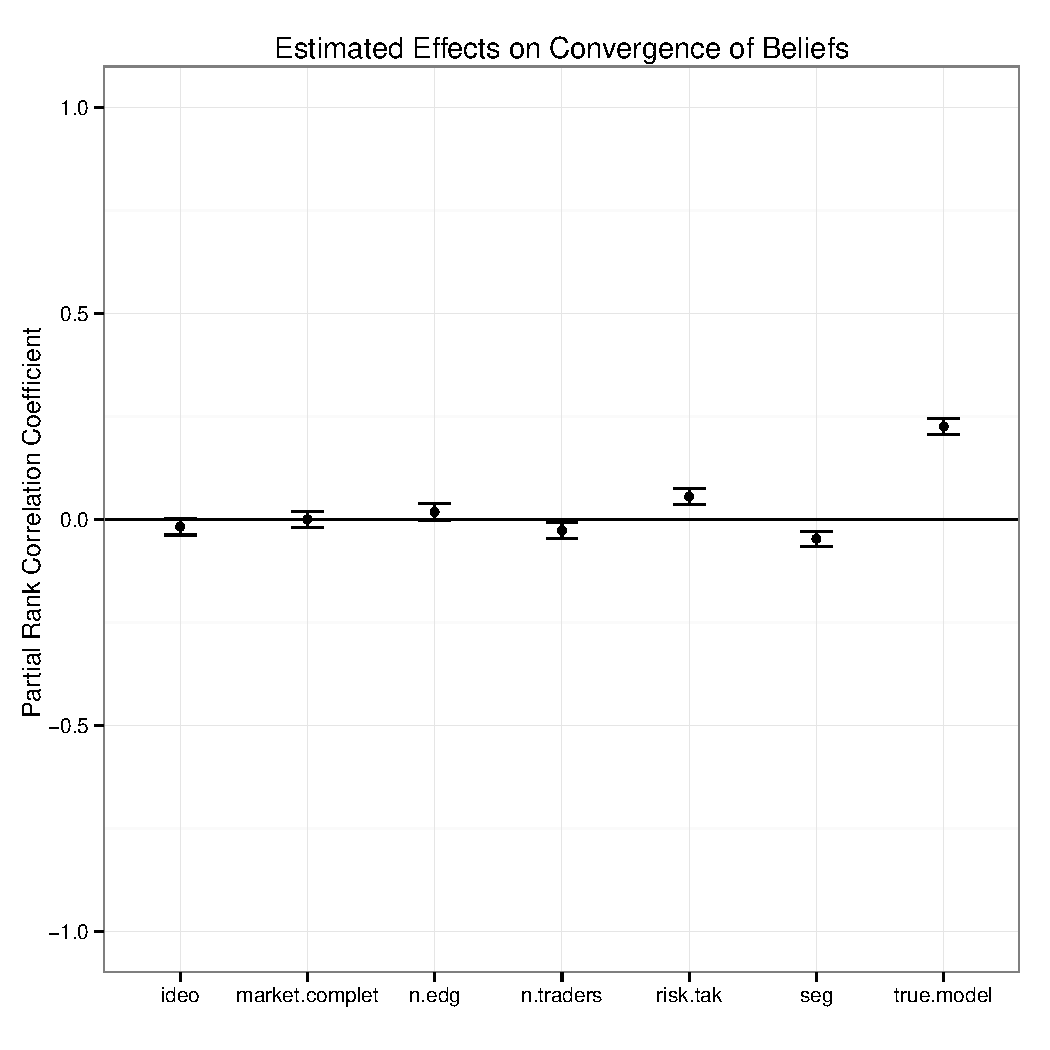
\includegraphics[width=\maxwidth]{figure/pc_sa-1} 

\end{knitrout}
\caption{Partial rank correlation coefficient analysis based on 10,000 simulated parameter sets \cite{pujol_sensitivity:_2014,saltelli_sensitivity_2009} of the effects of ideology, market completeness, number of edges in social network, number of traders in market, risk taking propensities, segregation measure of the social network, and the true climate model on the convergence of traders' beliefs. Lines are bootstrapped 95\% confidence intervals.}
\label{fig:pc_sa}
\end{figure}

\begin{figure}
\centering
\begin{knitrout}
\definecolor{shadecolor}{rgb}{0.969, 0.969, 0.969}\color{fgcolor}
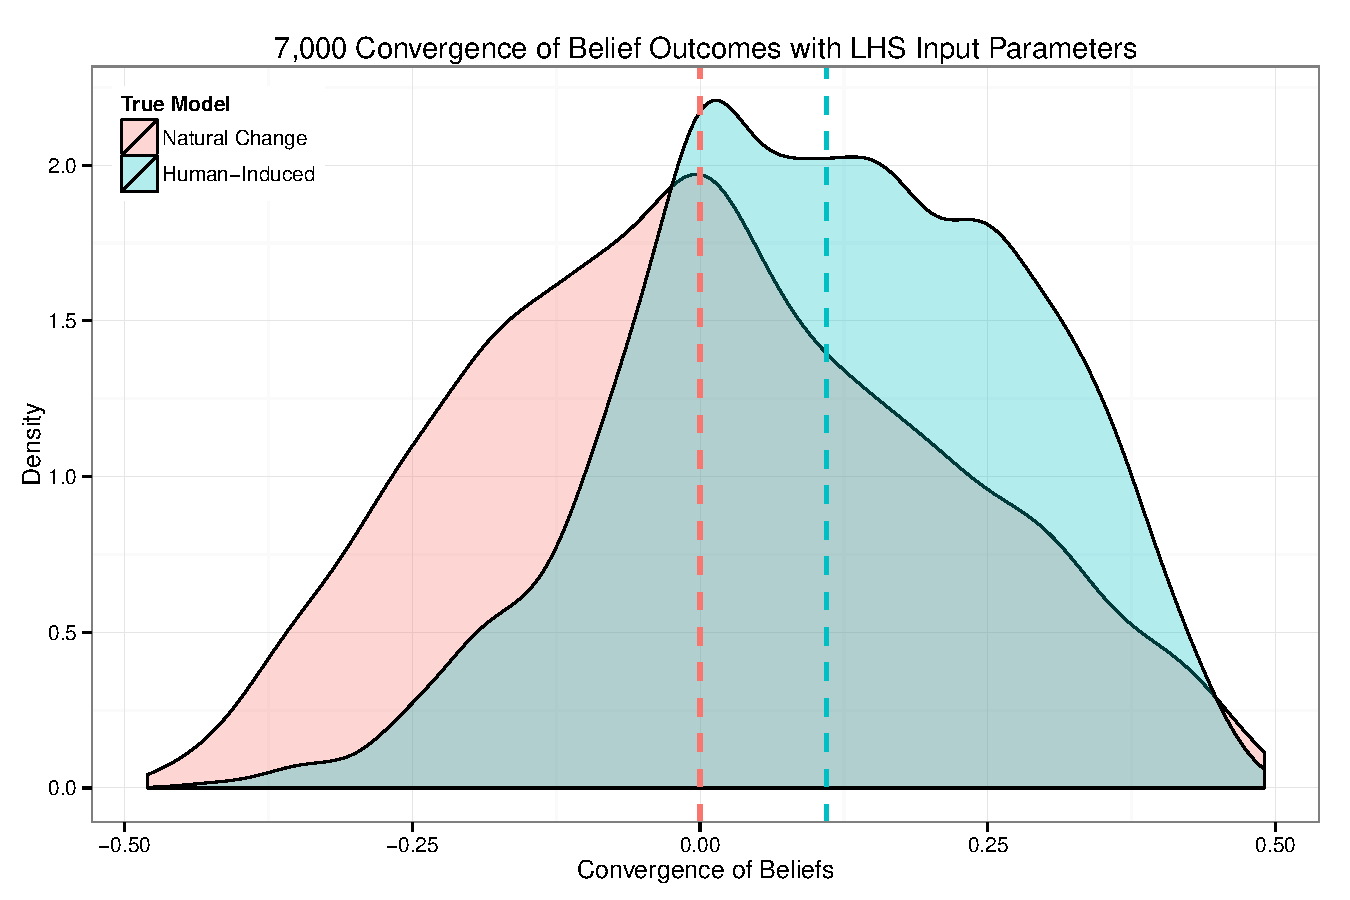
\includegraphics[width=\maxwidth]{figure/hist-1} 

\end{knitrout}
\caption{Density of 7,000 convergence of belief model outcomes with 7,000 Latin Hypercube Sampled input parameter sets. 3,500 of the Latin Hypercube Sampled input parameter sets have ``human-induced'' climate change as the true model and 3,500 have ``natural change'' climate change as the true model. Dashed lines are the medians of the two densities (0, 0.11). Possible values of convergence of beliefs range from -1 to 1.}
\label{fig:hist}
\end{figure}

\begin{figure}
\centering
\begin{knitrout}
\definecolor{shadecolor}{rgb}{0.969, 0.969, 0.969}\color{fgcolor}
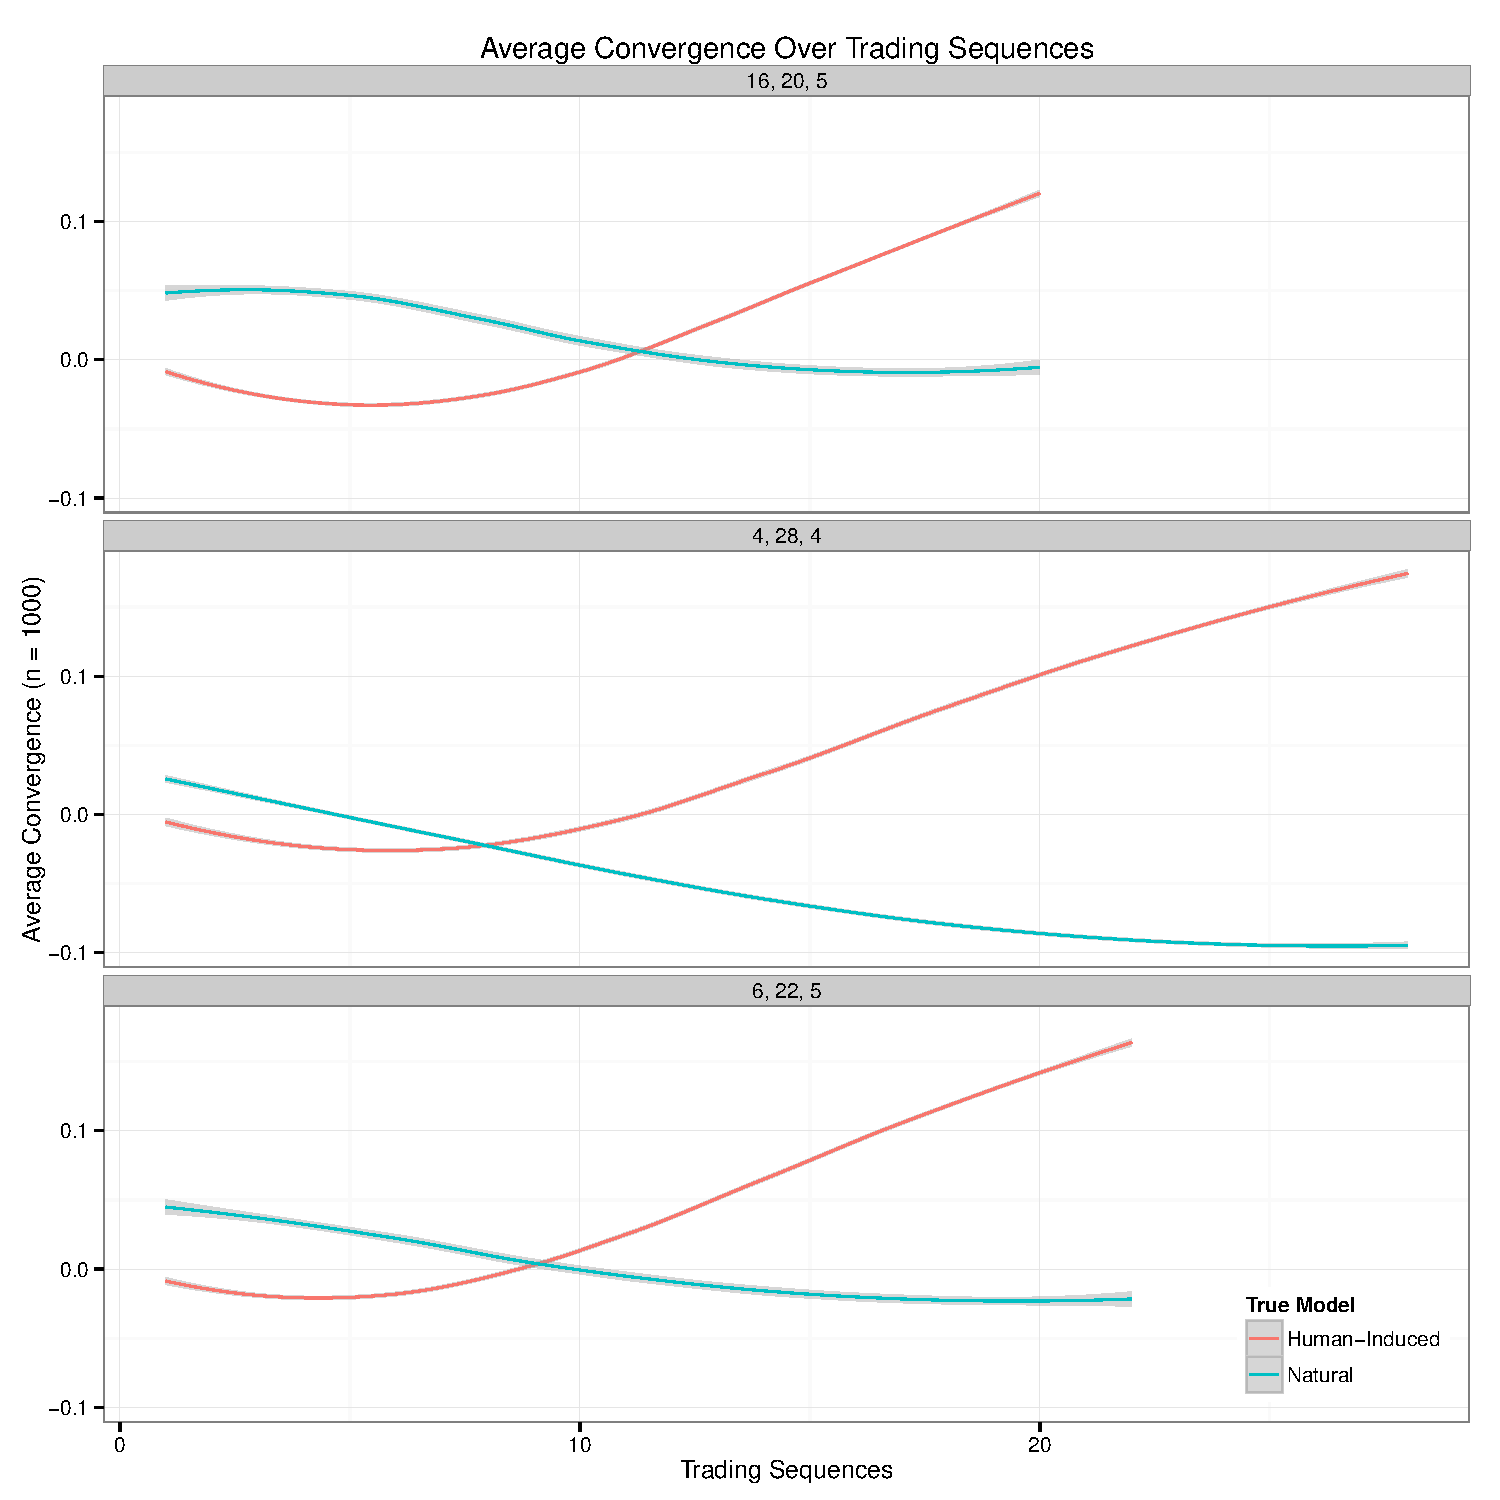
\includegraphics[width=\maxwidth]{figure/temporal-1} 

\end{knitrout}
\caption{Temporal evolution of convergence of beliefs for the ABM with 1,000 model runs with ``True Model'' parameter set to natural climate change and 1,000 model runs with ``True Model'' parameter set to human-induced climate change. All other parameters are sampled from their full support with Latin Hypercube Sampling; therefore, the plot represents, in effect, a marginalizing out of the effects of all other parameters to show the moderating effect that the true model has on the effect of the prediction market on the convergence of traders' beliefs about what the true model is. The prediction market causes opposite convergence effects for the two true climate models.}
\label{fig:temporal}
\end{figure}

%%%%%%%%%%%%%%%%%%%%%%%%%%%%%%%%%%%%%%%%%%%%%%%%%%%%%%%%%%%%%%%%%%%%%%%%%%%%%%%%
\section*{Discussion}
Proponents of climate prediction markets argue that climate prediction markets will foster convergence to the best approximate model, whatever the actual true model is. It is framed as an apartisan proposal: if climate change is not anthropogenic, traders will converge to non-anthropogenic beliefs similar to how they would converge to anthropogenic beliefs if the climate is truly influenced by human activities. Our findings contradict this assumption. 

TODO: Jonathan, perhaps talk about the policy implications of this finding...

%%%%%%%%%%%%%%%%%%%%%%%%%%%%%%%%%%%%%%%%%%%%%%%%%%%%%%%%%%%%%%%%%%%%%%%%%%%%%%%%
\section*{Acknowledgements}
We gratefully acknowledge the authors of \textsf{R} \cite{r_core}. This manuscript was prepared using knitr \cite{xie_knitr_2014} and benefited from our exposure to the literature on reproducible research \cite{stodden_reproducible_research_2014}. We would like to thank Yevgeniy Vorobeychik for feedback on this project.

%%%%%%%%%%%%%%%%%%%%%%%%%%%%%%%%%%%%%%%%%%%%%%%%%%%%%%%%%%%%%%%%%%%%%%%%%%%%%%%%
\bibliographystyle{plain}
\bibliography{library}

%%%%%%%%%%%%%%%%%%%%%%%%%%%%%%%%%%%%%%%%%%%%%%%%%%%%%%%%%%%%%%%%%%%%%%%%%%%%%%%%
\end{document}
